\documentclass[12pt,letterpaper]{article}
\usepackage{fullpage}
\usepackage[top=2cm, bottom=4.5cm, left=2.5cm, right=2.5cm]{geometry}
\usepackage{amsmath,amsthm,amsfonts,amssymb,amscd}
\usepackage{lastpage}
\usepackage{enumerate}
\usepackage{fancyhdr}
\usepackage{hyperref}
\usepackage{pythontex}
\usepackage[siunitx]{circuitikz}
\usepackage{xcolor}
\usepackage[inline]{enumitem}
\usepackage{booktabs}
\usepackage{relsize}
\usepackage{calculator}
\usepackage{siunitx}

\setlength{\parindent}{0.0in}
\setlength{\parskip}{0.05in}

% Edit these as appropriate
\newcommand\course{MCEN 5228-004}
\newcommand\project{1}                  % <-- homework number
\newcommand\NetIDa{Coovi Meha}           % <-- NetID of person #1
\newcommand\NetIDb{MEid:481-473}           % <-- NetID of person #2 (Comment this line out for problem sets)

\pagestyle{fancyplain}
\headheight 35pt
\lhead{\NetIDa}
\lhead{\NetIDa\\\NetIDb}                 % <-- Comment this line out for problem sets (make sure you are person #1)
\chead{\textbf{\Large Project \project}}
\rhead{\course \\ \today}
\lfoot{}
\cfoot{}
\rfoot{\small\thepage}
\headsep 1.5em
\begin{document}
\begin{pycode}
R=5100
C=2.2*10**-6
tau=2/(R*C)
tau1=0.5*tau
omega=tau**0.5
\end{pycode}
\section*{Abstract}
In system analysis, engineer study the performance of a system using theoretical and 
experimental approaches. However, most system do not perform as  predicted by the theoretical model. Thus, the need to make adjustment to the model using experimental data.
In the following experiments, we study both theoretically and experimentally the performance of an RRC circuit. The data colleted from the experiment would then used correct the theoretical system parameter to match a real 
life situation if possible.
\section*{Backgrounds}
This experiment used an RRC circuit as showed bellow. 
\begin{figure}[h]
    \begin{center}
        \begin{circuitikz}\draw
            (0,0) to[battery, color=red] (0,4) 
            to[R=5.1<k\ohm>] (4,4) to [R=5.1<k\ohm>] (4,0)
            --(0,0) 
            (4,4) -- (6,4) to[capacitor, C=2.2<\micro\farad>, color=blue] (6,0) 
            -- (4,0) 
            (6,4)  to[short,-*] (8,4) 
            (8,0) to[open, v=${V_out}$, color=red] (8,4) 
            (6,0)  to[short,-*] (8,0) 
            ;
        \end{circuitikz}
        \caption{RRC Circuit}
        \end{center}
\end{figure}
we were interested in measuring the voltage crossing the capacitor and the resistor in parallel.
The measure voltage is compared to the input voltage in oder to analyse the gain of the system, the rise time of, the settle time and others parameters associated
the input-output signal. 

The system was fed with two difference signal:
\begin{itemize}
    \item A step input signal of 1 volt
    \item A sinusoidal input of amplitude 1 volt, phase of zero degree and 10 Hzt frequency 
\end{itemize}
\section*{Theoretical Results}
\begin{itemize}
    \item Idealize Elements
    
    \begin{circuitikz}\draw
        (0,0) node[{label=above:$V_{in}$}]{} to [R=$R$, *-*] node[{label=above:$V_{1}$}]{}(4,0)
        (5,0) node[{label=above:$V_{2}$}]{}to [capacitor=$C$, *-*] node[{label=above:$V_{3}$}]{}(9,0)
         (10,0) node[{label=above:$V_{4}$}]{} to [R=R, *-*] node[{label=above:$V_{5}$}]{}(14,0);
    \end{circuitikz}
    \item  Derivation of Transfer Function and Time Domain Equation
    
    From the Idealized element, the idealized formula can be derived as follow.


        \begin{enumerate*}
            \item \(V_{in}-V_{1}= R*I\) \quad \quad \quad \quad
            \item \(V_{2}-V_{3}=\frac{1}{C}*I_{2}\) \quad \quad \quad \quad
            \item \(V_{4}-V_{5}= R*I\) \quad \quad \quad \quad
            \item \(V_{1}=V_{2}=V_{4}=V_{out}\) \quad \quad \quad \quad
            \item \(V_{3}=V_{5}=0\)
        \end{enumerate*}


    From the above equations: 

    \begingroup
    \Large
    \begin{equation}
        H(s)=\frac{1}{2}  *\frac{\frac{2}{RC}}{s+ \frac{2}{RC}} \quad \equiv \quad H(s)=\frac{\py{round(tau1,2)}}{s+ \py{round(tau,2)}}
    \end{equation}
    \endgroup
    with R=5.1k \({\Omega}\) and C=2.2 \(\si{\micro\farad}\)
    The laplace inverse of the equation (1) leads to:
    \begingroup
    \Large
        \begin{equation}
            y(t)=\frac{1}{2}({1} - e^{\frac{-2t}{CR}})
        \end{equation}
    \endgroup
    \item Analysis of Performance 
    \begin{enumerate}
        \item From equation (1), the gain of system is 0.5
        \item \({\omega}_n^2={(\frac{2}{RC})}^2\)
        \item On a step input using Matlab, the rise time of the system is 12.3 ms
        and settle time is 0.0219 s . Base on the equation (1), we can conclude that
        the system has a cut off frequency at \(\omega_c = \py{round(omega,2)}\) rad/s and steady state error of 0.5.
        \begin{figure}[h]
            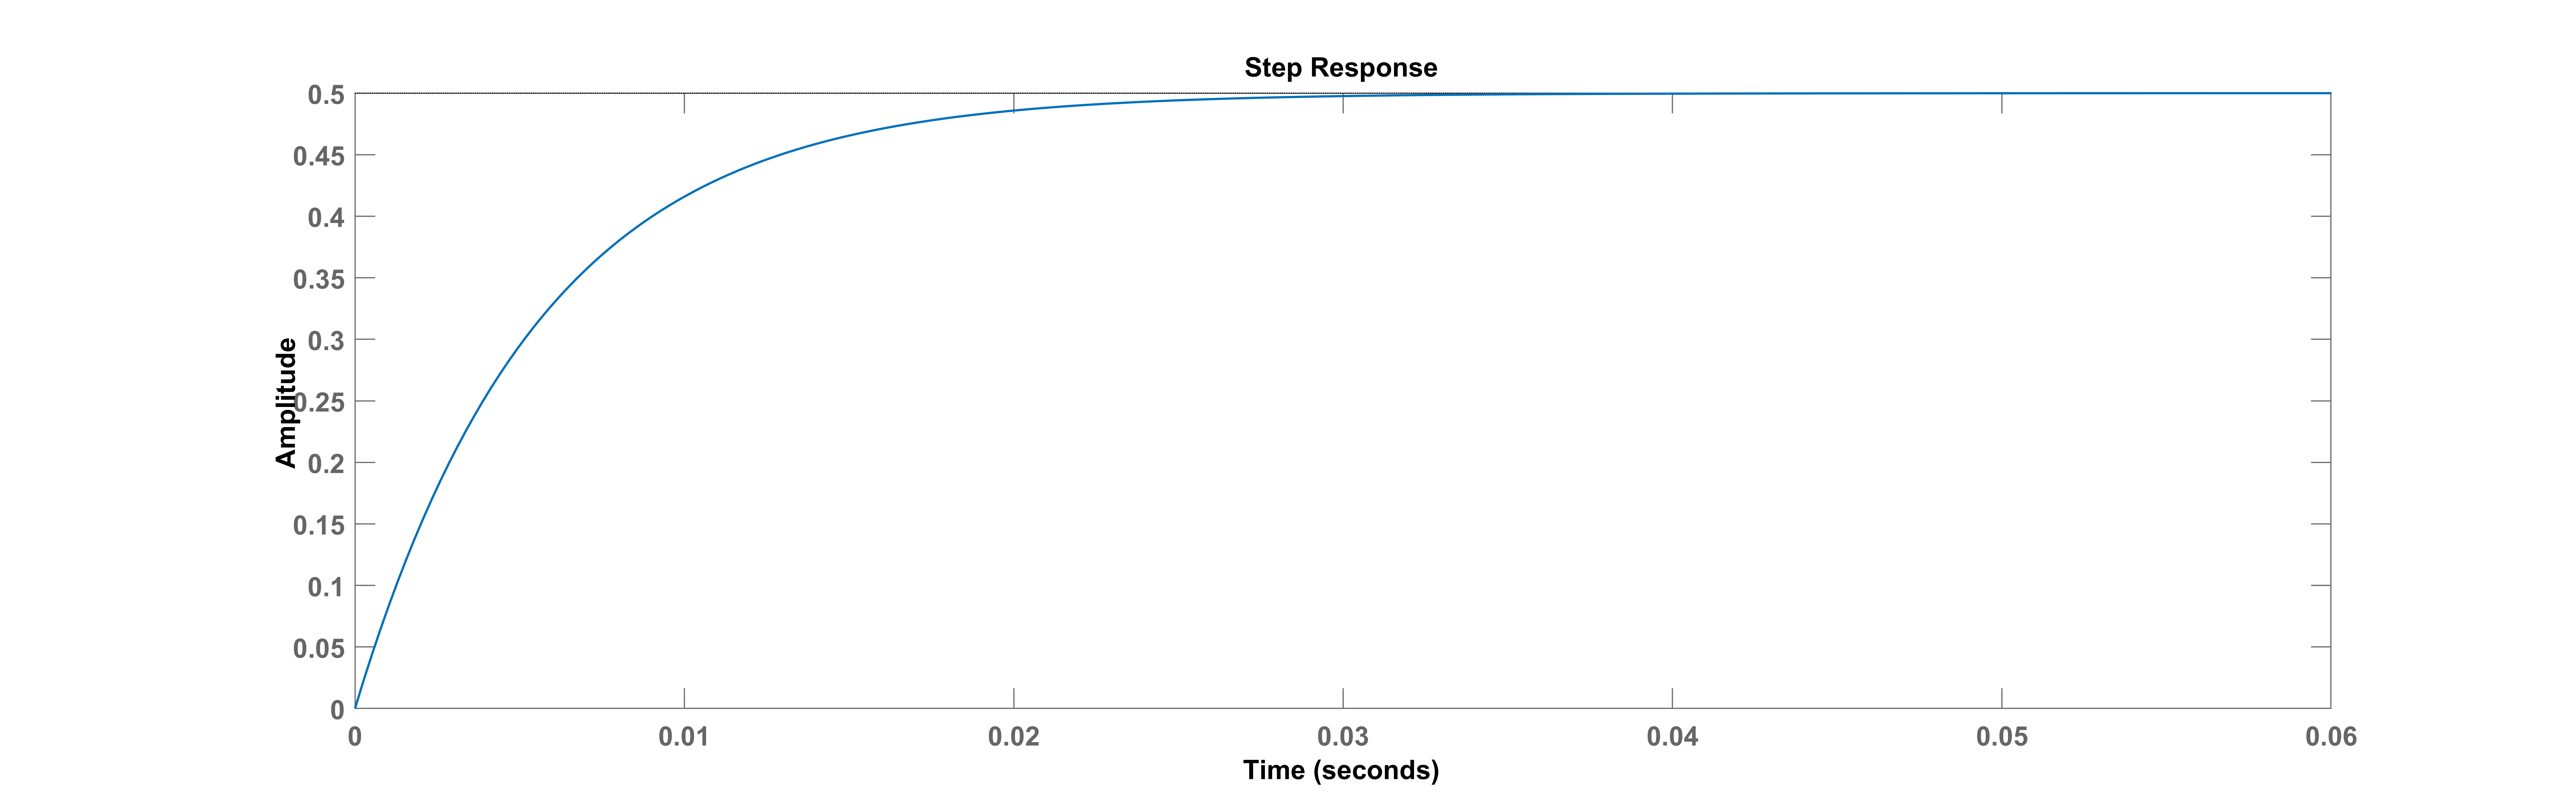
\includegraphics[width=17cm]{sep_theory.png}
            \caption{Plot of step input response of 1 volt to RRC circuit using Matlab}
        \end{figure}
        \item On a sinusoidal input of frequency 10Hz and amplitude 1such that \(x(t)=sin(20{\pi}t)\)
        using Matlab control package lsim(), it is seen as showed in the following figure 
        that the amplitude of the output signal is 0.47 and has phase shift of 19.4 degrees
        \begin{figure}[h]
            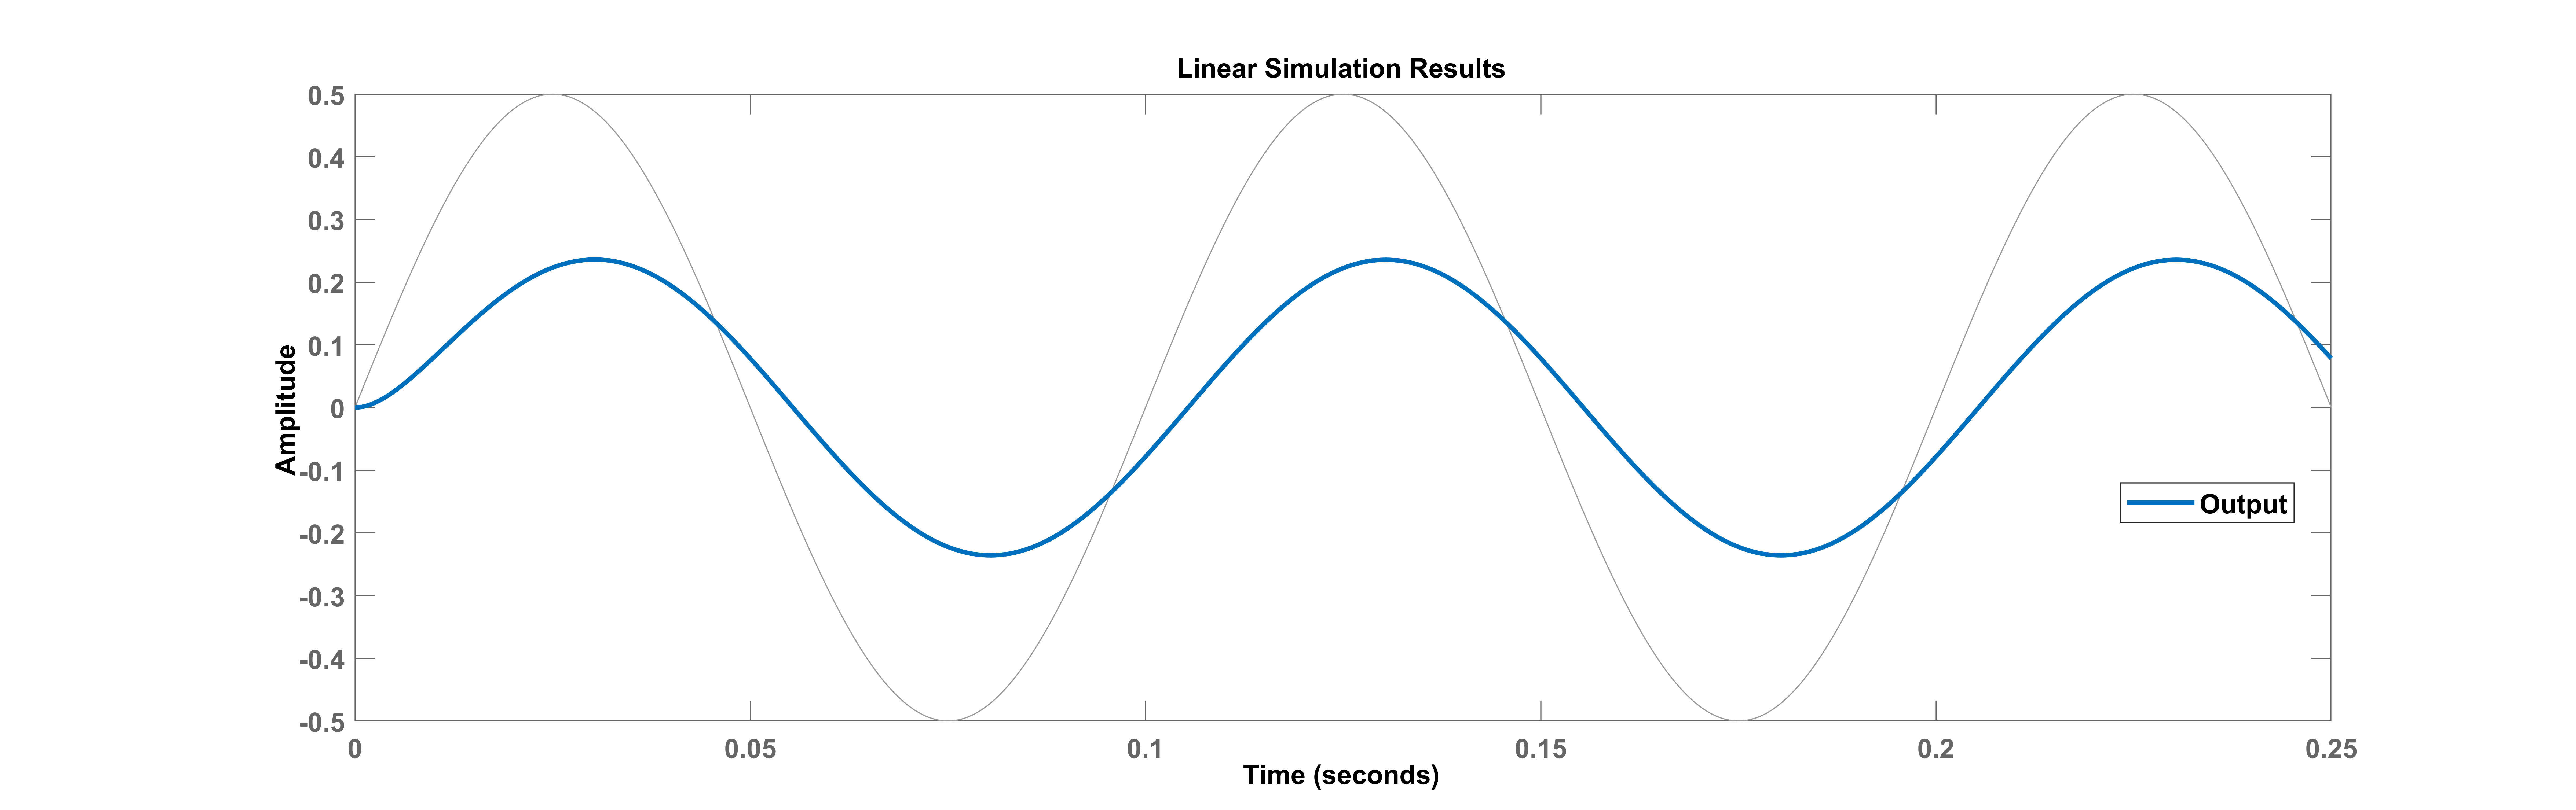
\includegraphics[width=17cm]{wave_theory.png}
            \caption{Plot sin input signal of 10Hz }
        \end{figure}
        The phase shift was found using the bode plot of the transfer function to 
        estimate the phase at the 62.8 rad/s as shown bellow.
        \begin{figure}[h]
            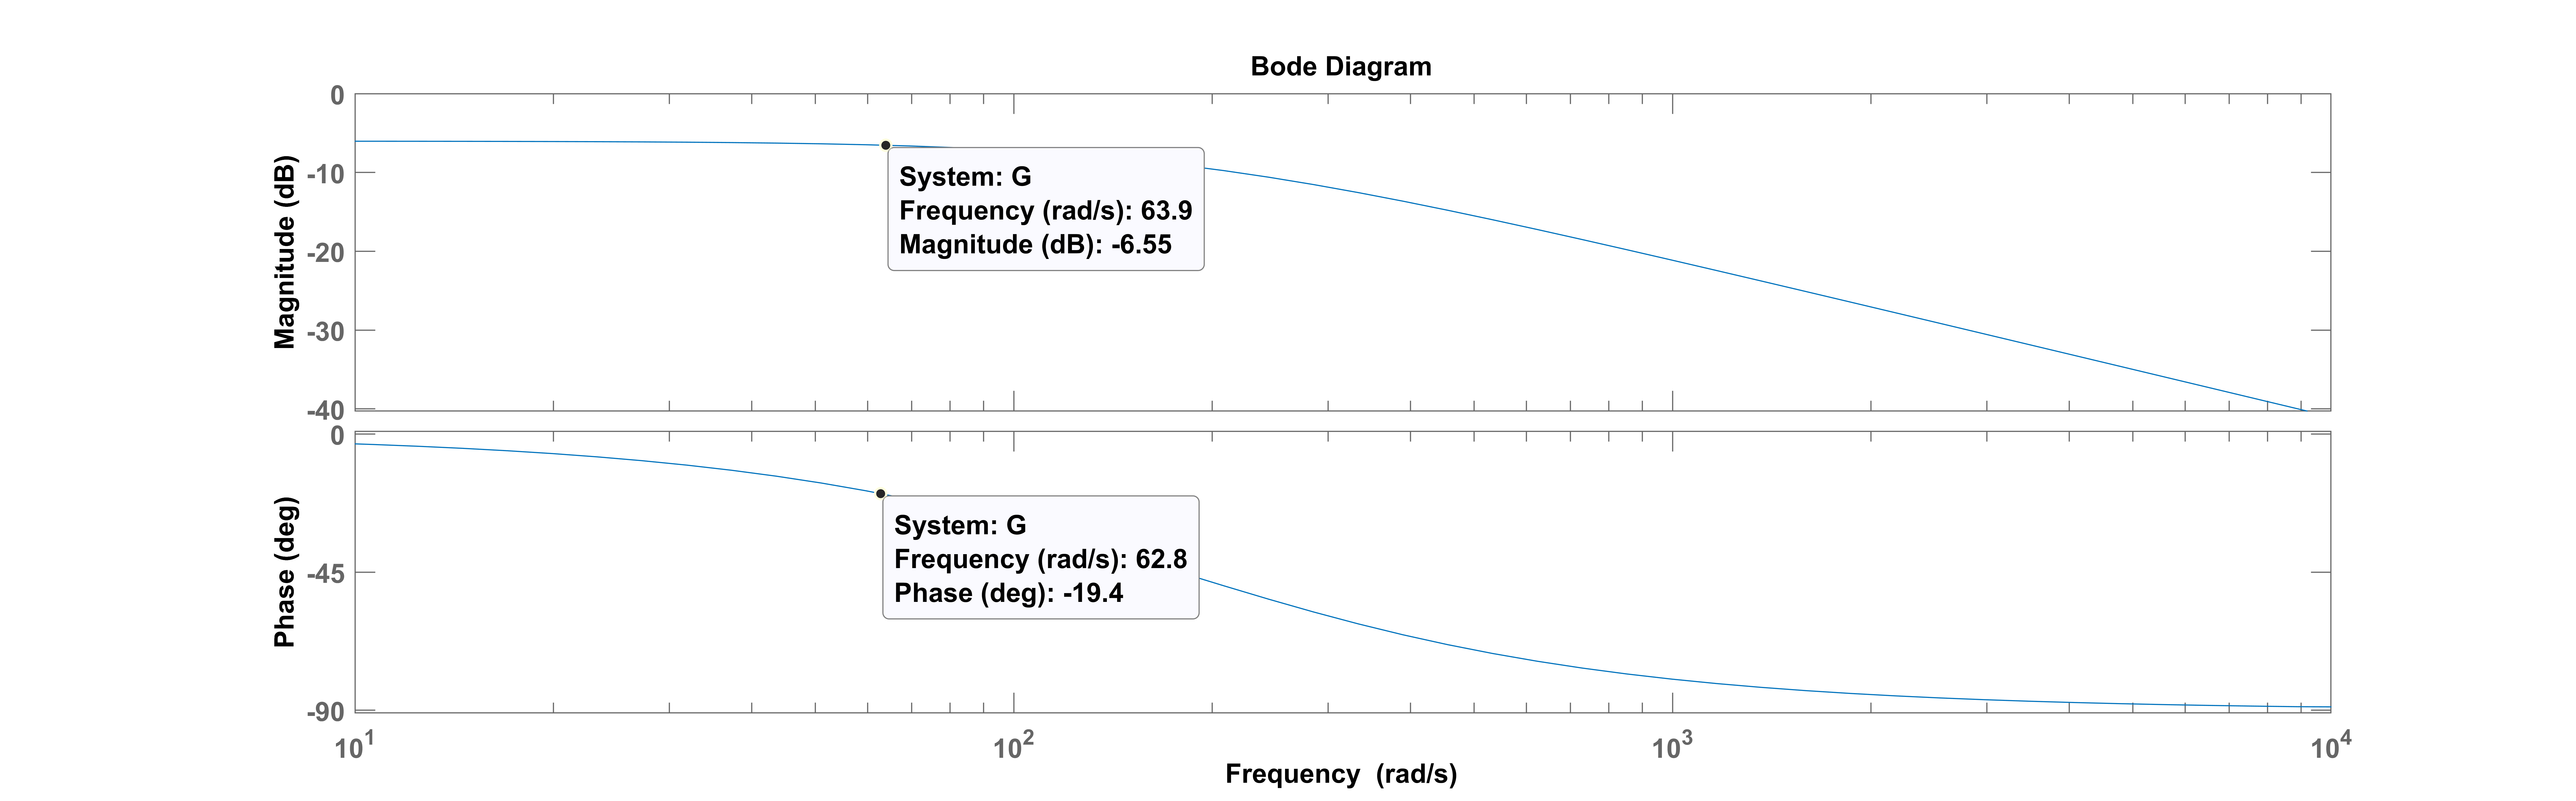
\includegraphics[width=17cm]{bode_plot.png}
            \caption{Bode plot of equation(2) showing phase shift at 10Hz}
        \end{figure}
    \end{enumerate}
\end{itemize}
\section*{Experimental Results} 
\begin{enumerate}
    \item Step Input
    
    on step input, it was notice that the gain of the system from the oscilloscope
    was about .52V and the rise time of the system output is 10.85 ms.\\
    \begin{figure}[h]
        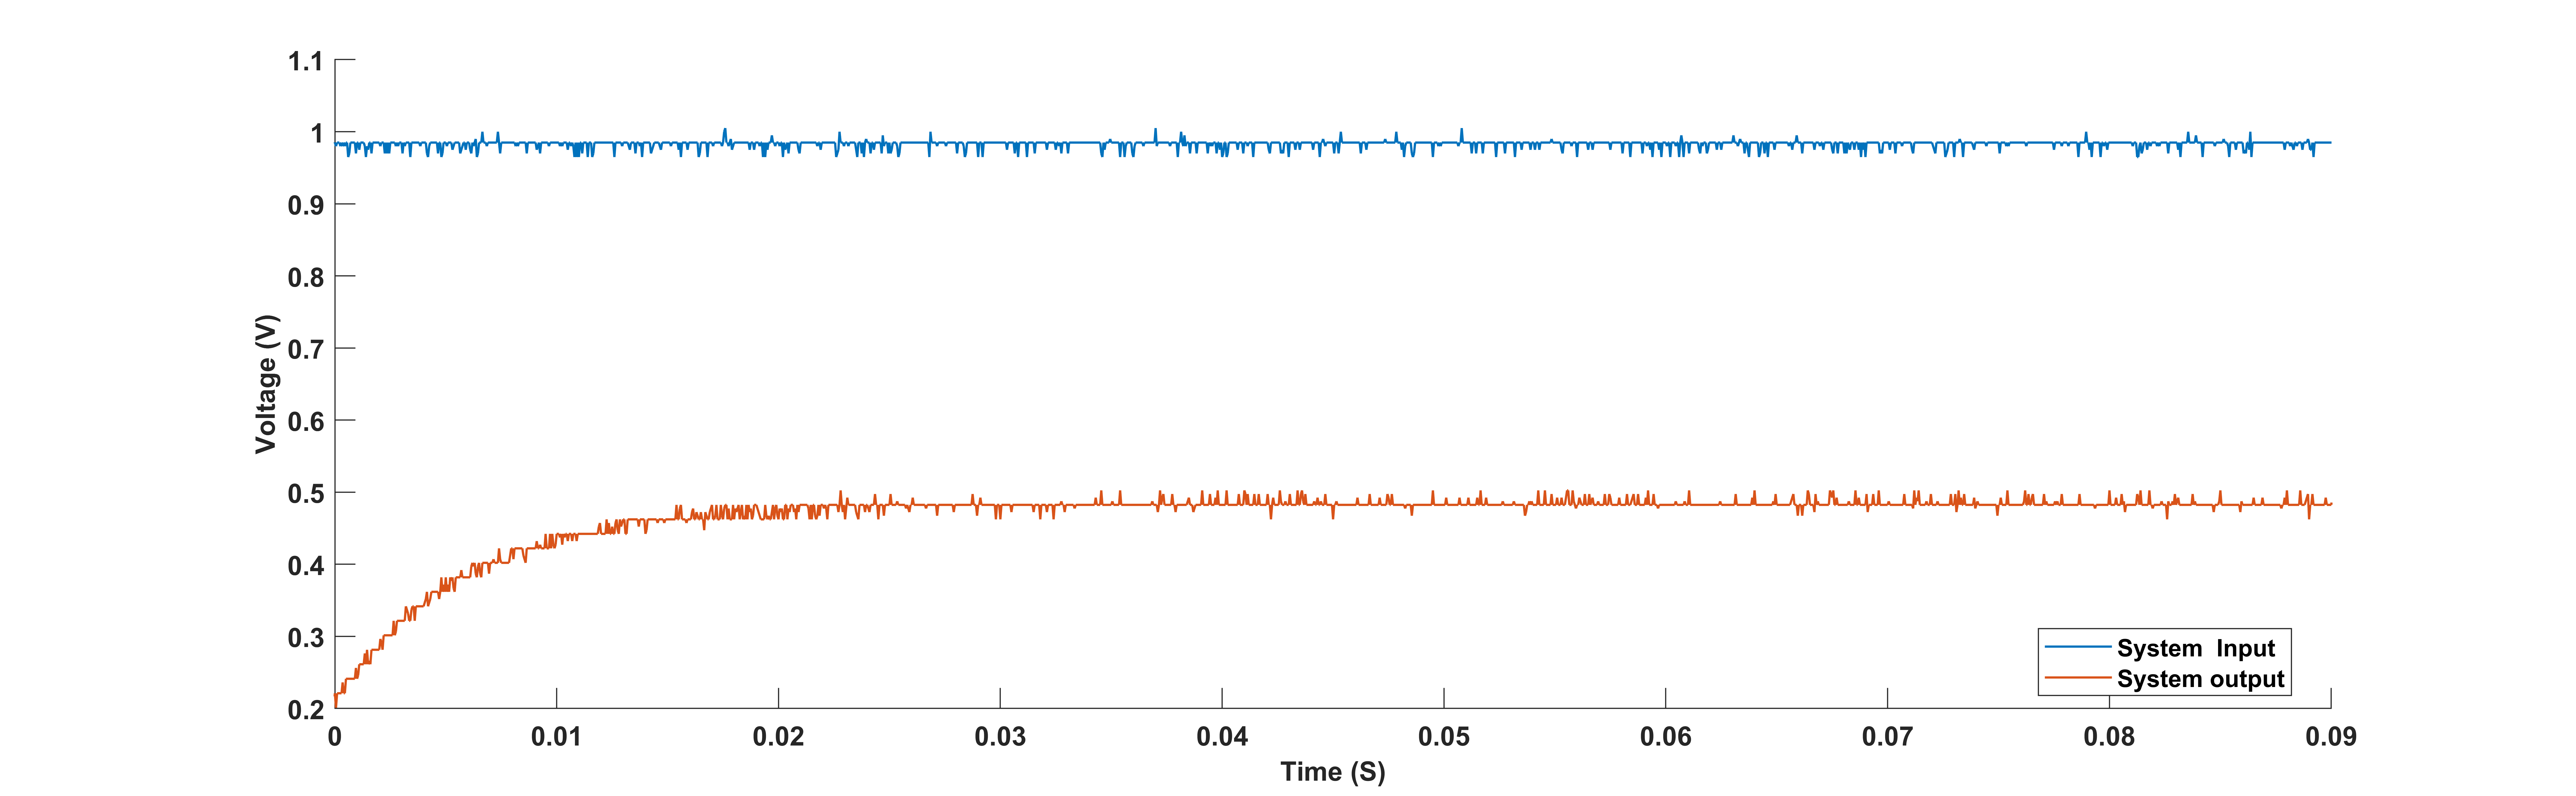
\includegraphics[width=17cm]{sep_exp.png}
        \caption{Experimental plot of step input of 1 volt to an RRC circuit.}
    \end{figure}
    \item Sin Input of 10Hz\\
    On the input of 10Hz, it was recorded that the system output has a pick to pick voltage of 
    .52 volts and and a phase shift of -19.22 degrees.
    \begin{figure}[h]
        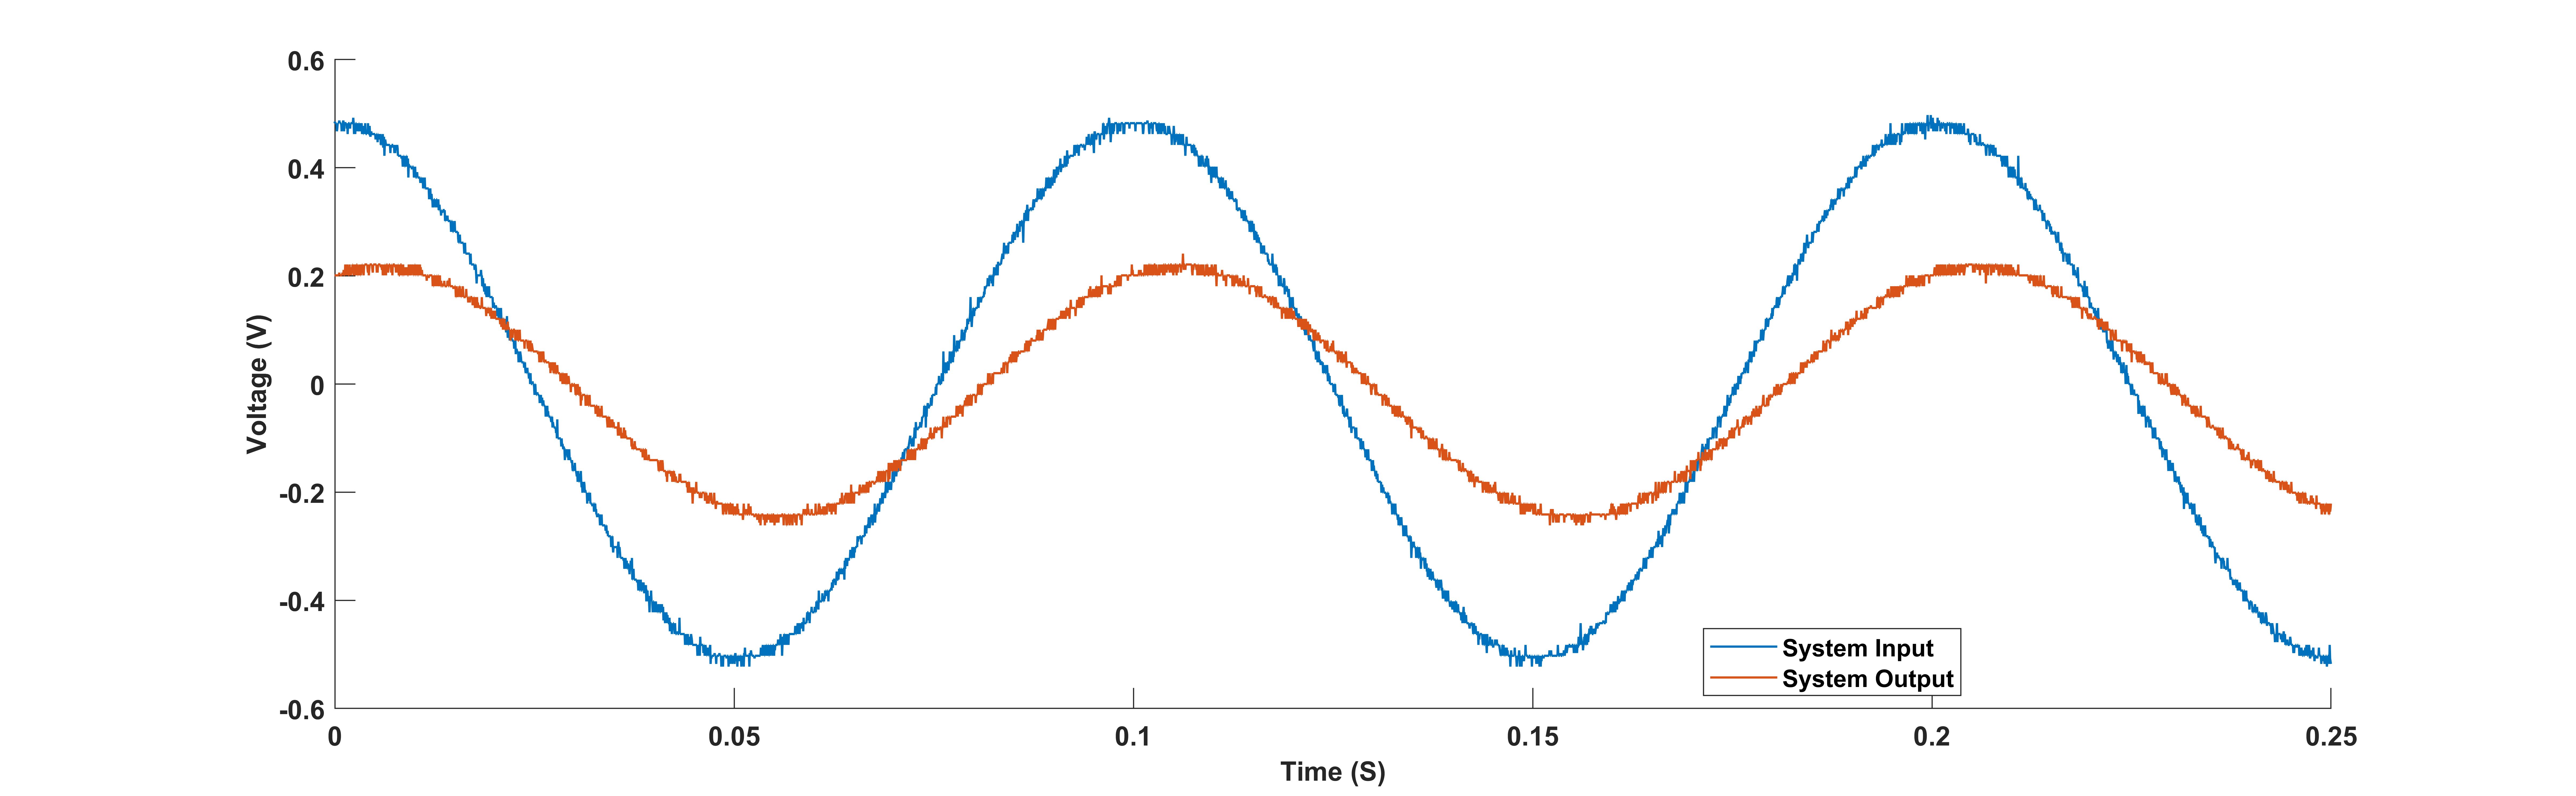
\includegraphics[width=17cm]{wave_exp.png}
        \caption{Experimental plot of sin input of 10Hz and amplitude 1V to an RRC circuit.}
    \end{figure}
\end{enumerate}
\section*{Parameters Adjustment}
To make correct the values of the resistor and the capacitor used in this experiment in the theory
to fit the experimental results, it is critical to work in the time domain not in the laplace nor frequency domain
    To the step input, using inverse laplace function  from Matlab, the time domain output function  is:\\
    \begingroup
    \Large
    \begin{equation}
        y(t)=\frac{1}{2}({1} - e^{\frac{-2t}{CR}})
    \end{equation}
    \endgroup
    In oder to have reproduce the gain of the experimental result, it is convenient to find 
    new values of the resistance and capacitor in this circuit. Do to so, the output discrete data can 
    fitted to the theoretical equation(3) in matlab to get the new value of R and C. \\
    Using Matlab fitting capability, the new R values found is 5.5\(k{\Omega}\) and the capacitance is 2.44\(\si{\micro\farad}\)

\section*{Conclusion}
Looking at the theoretical and experimental result, it can be said that the system has a worse. 
performance overall of about 50 percent error. However, experimental and the theoretical result 
are well correlated. For the step input, the gain of the system is .5 theoretically and .48 experimentally.
Thus, an error of 4 percentage. With an error bellow 5 percent, it reasonable not to correct the
the parameter of the system because any correction would not bring about significant improvement.\\
For the sin input, it could be seen that the pick to pick voltage of the output wave is 5.2 experimentally and 4.8 theoretically. The 
phase was shift fot about 19.44 degrees in theory versus 19.22 degree during the experiment.
The error associated are  8 percent for the pick to pick voltage and 11 percent for the phase or 0.22 degree. \\
The error seen during this experiment could be due to the tolerance set on the resistor or the capacitor. 
Using a millimeter to manually check the capacitance of reveal that C=3.0 \(\si{\micro\farad}\) and the resistor had a resistance of 
R=4.99 \(k{\Omega}\). 
\end{document}

